\documentclass[10pt,a4paper]{article}
\usepackage[utf8]{inputenc}
\usepackage[ngerman]{babel}
\usepackage[T1]{fontenc}
\usepackage{amsmath}
\usepackage{amsfonts}
\usepackage{amssymb}
\usepackage{graphicx}
\usepackage{lmodern}
\usepackage{physics}
\usepackage[left=1cm,right=1cm,top=1.5cm,bottom=1.2cm]{geometry}
\usepackage{siunitx}
\usepackage{fancyhdr}
\usepackage{enumerate}
\usepackage{mhchem}
\usepackage{mathtools}
\usepackage{graphicx}
\usepackage{float}
\usepackage{xcolor}
\usepackage{mdframed}
\usepackage{csquotes}
\usepackage{trfsigns}
\usepackage{capt-of}
\usepackage{minted}

\sisetup{locale=DE}
\sisetup{per-mode = symbol-or-fraction}
\sisetup{separate-uncertainty=true}
\DeclareSIUnit\year{a}
\DeclareSIUnit\clight{c}
\mdfdefinestyle{exercise}{
	backgroundcolor=black!10,roundcorner=8pt,hidealllines=true,nobreak
}

\begin{document}
\twocolumn
\pagestyle{fancy}
\lhead{DSP Formelsammlung, \today}
\rhead{Sedlmeier, Toni}
\section{Zahlenformate}
\begin{center}
  \includegraphics[width=.5\textwidth]{./img/dynamic.png}
\end{center}
%%%%%%%%%%%%%%%%%%%%%%%%%%%%%%%%%%%%%%%%%%%%% Zahlenformate %%%%%%%%%%%%%%%%%%%%%%%%%%%%%%%%%%%%%%%%%%%%%%%%%%%%%
  \subsection{Zweierkomplement}
  Umwandlung: Bsp. 8-Bit $(-4)_{10}$ (Funktioniert in beide Richtungen)
  \begin{itemize}
      \item Vorzeichen Ignorieren $(4)_{10} = (0000 0100)_2$
      \item Bits Invertieren $(0000 \ 0100)_2 \ \rightarrow (1111\ 1011)_2$
      \item Eins Addieren $(1111\ 1011)_2 + (0000\ 0001)_2 = (1111\ 1100)_2$
  \end{itemize} 
  \subsection{Fixed Point (unsigned)}
Qk.l mit k = Vorkomma und l = Nachkomma
  \begin{mdframed}[style=exercise]
    \begin{align}
        x_{(10)} = \sum_{i=0}^{k-1} b_i\cdot 2^i + \sum_{j=-l}^{-1} b_j\cdot 2^j
    \end{align}
  \end{mdframed}
Bsp Q4.5 $a=(0101 0110)_2$ \\
$\textcolor{red}{0}\cdot 2^3+\textcolor{red}{1}\cdot 2^2+\textcolor{red}{0}\cdot 2^{1}+\textcolor{red}{1}\cdot 2^0+\textcolor{red}{0}\cdot 2^{-1}+\textcolor{red}{1}\cdot 2^{-2}+\textcolor{red}{1}\cdot 2^{-3}+\textcolor{red}{0}\cdot 2^{-4}=5.375$

  \subsection{Fixed Point (signed)}
Bsp. Q3.3 $(100.001)_2$ 
  \begin{itemize}
      \item Vorzeichen Merken (\textcolor{red}{1}00.001) $\rightarrow \ \textcolor{red}{-1}$
      \item Bits Invertieren $(100 \ 001)_2 \ \rightarrow (011\ 110)_2$
      \item $1\cdot 2^{-k}$ Addieren $(011\ 110)_2 + (000\ 001)_2 = (011\ 111)_2 = -3.875$
  \end{itemize} 

%%%%%%%%%%%%%%%%%%%%%%%%%%%%%%%%%%%%%%%%%%%%% Filter in c %%%%%%%%%%%%%%%%%%%%%%%%%%%%%%%%%%%%%%%%%%%%%%%%%%%%%
%%%%%%%%%%%%%%%%%%%%%%%%%%%%%%%%%%%%%%%%%%%%%  FIR %%%%%%%%%%%%%%%%%%%%%%%%%%%%%%%%%%%%%%%%%%%%%%%%%%%%%
\section{Filter in C}
\subsection{FIR}
\subsubsection{Blockschaltbild und math. Zusammenhänge:}
\begin{center}
  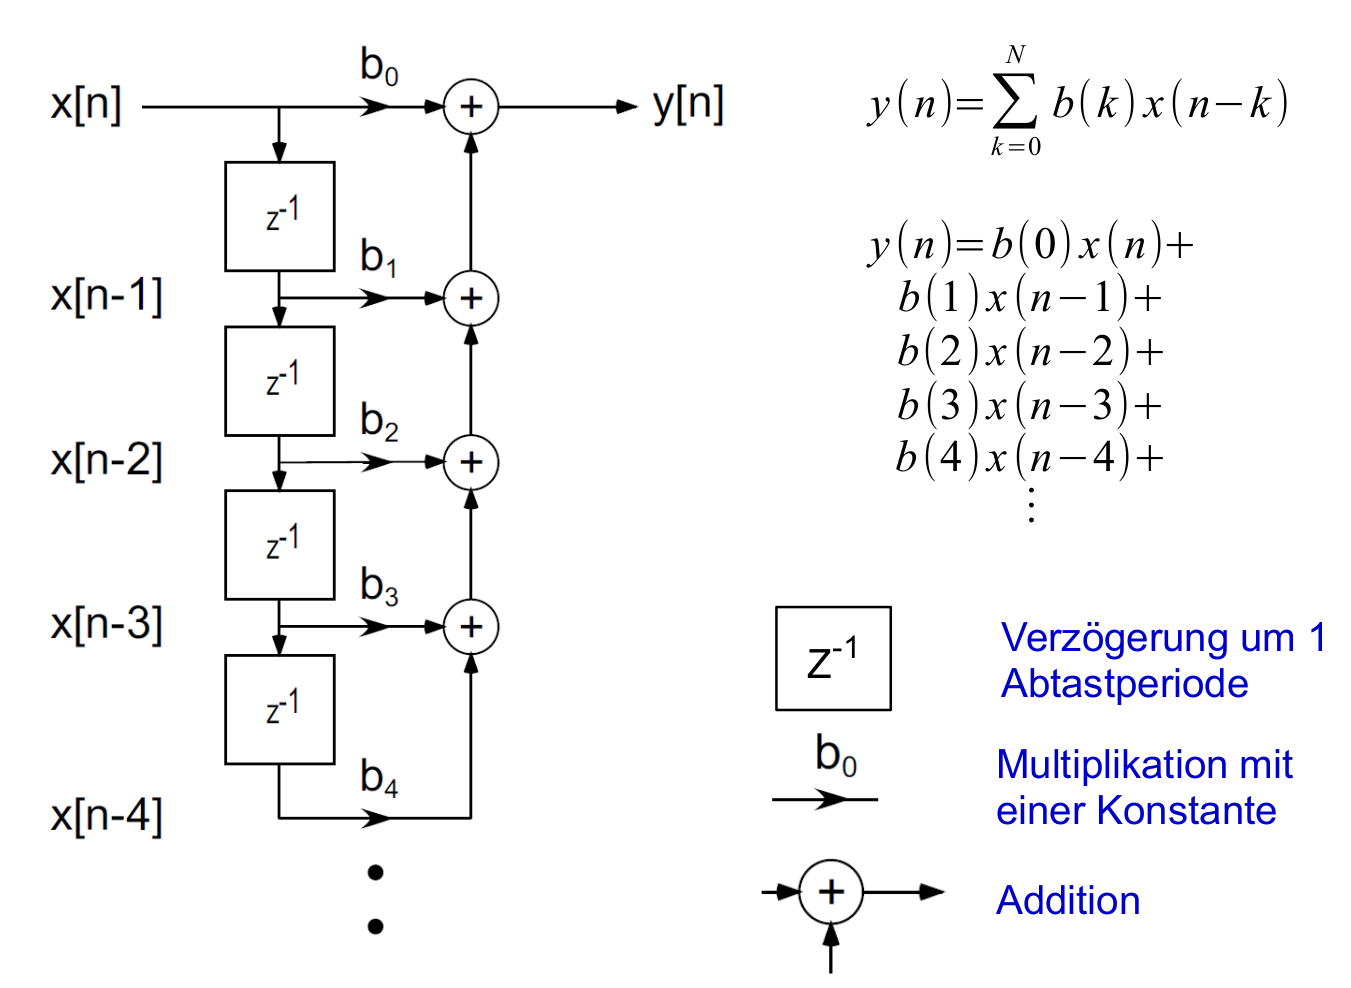
\includegraphics[width=.3\textwidth]{./img/FIR_Blockschaltbild.png}  
\end{center}

  \begin{mdframed}[style=exercise]
    \begin{align}
        A(0)y(k)=\sum_{i=0}^{N} B(i) x(k-i) 
    \end{align}
  \end{mdframed}

 \subsubsection{Realisierung des FIR in C:} 
\begin{minted}[fontsize=\scriptsize]{c}
void fir()
{
    CodecDataIn.UINT = ReadCodecData();     // get input data samples
    int i;
    xLeft[0] = CodecDataIn.Channel[LEFT];   // current input value
    yLeft = 0 ;                             // initialize the output
    for ( i = 0 ; i <= N ; i++) {           // x is length N+1
        yLeft += xLeft[i] * B[i];           // perform the dot-product
    }
    for ( i = N ; i > 0 ; i--) {
        xLeft[i] = xLeft[i-1];              // shift for the next input
    }
    CodecDataOut.Channel[LEFT] = yLeft;     // output the value
}
\end{minted}
%%%%%%%%%%%%%%%%%%%%%%%%%%%%%%%%%%%%%%%%%%%%%  IIR %%%%%%%%%%%%%%%%%%%%%%%%%%%%%%%%%%%%%%%%%%%%%%%%%%%%%
\subsection{IIR}
\subsubsection{Blockschaltbild und math. Zusammenhänge:}

\textbf{Direktform I:}
\begin{center}    
  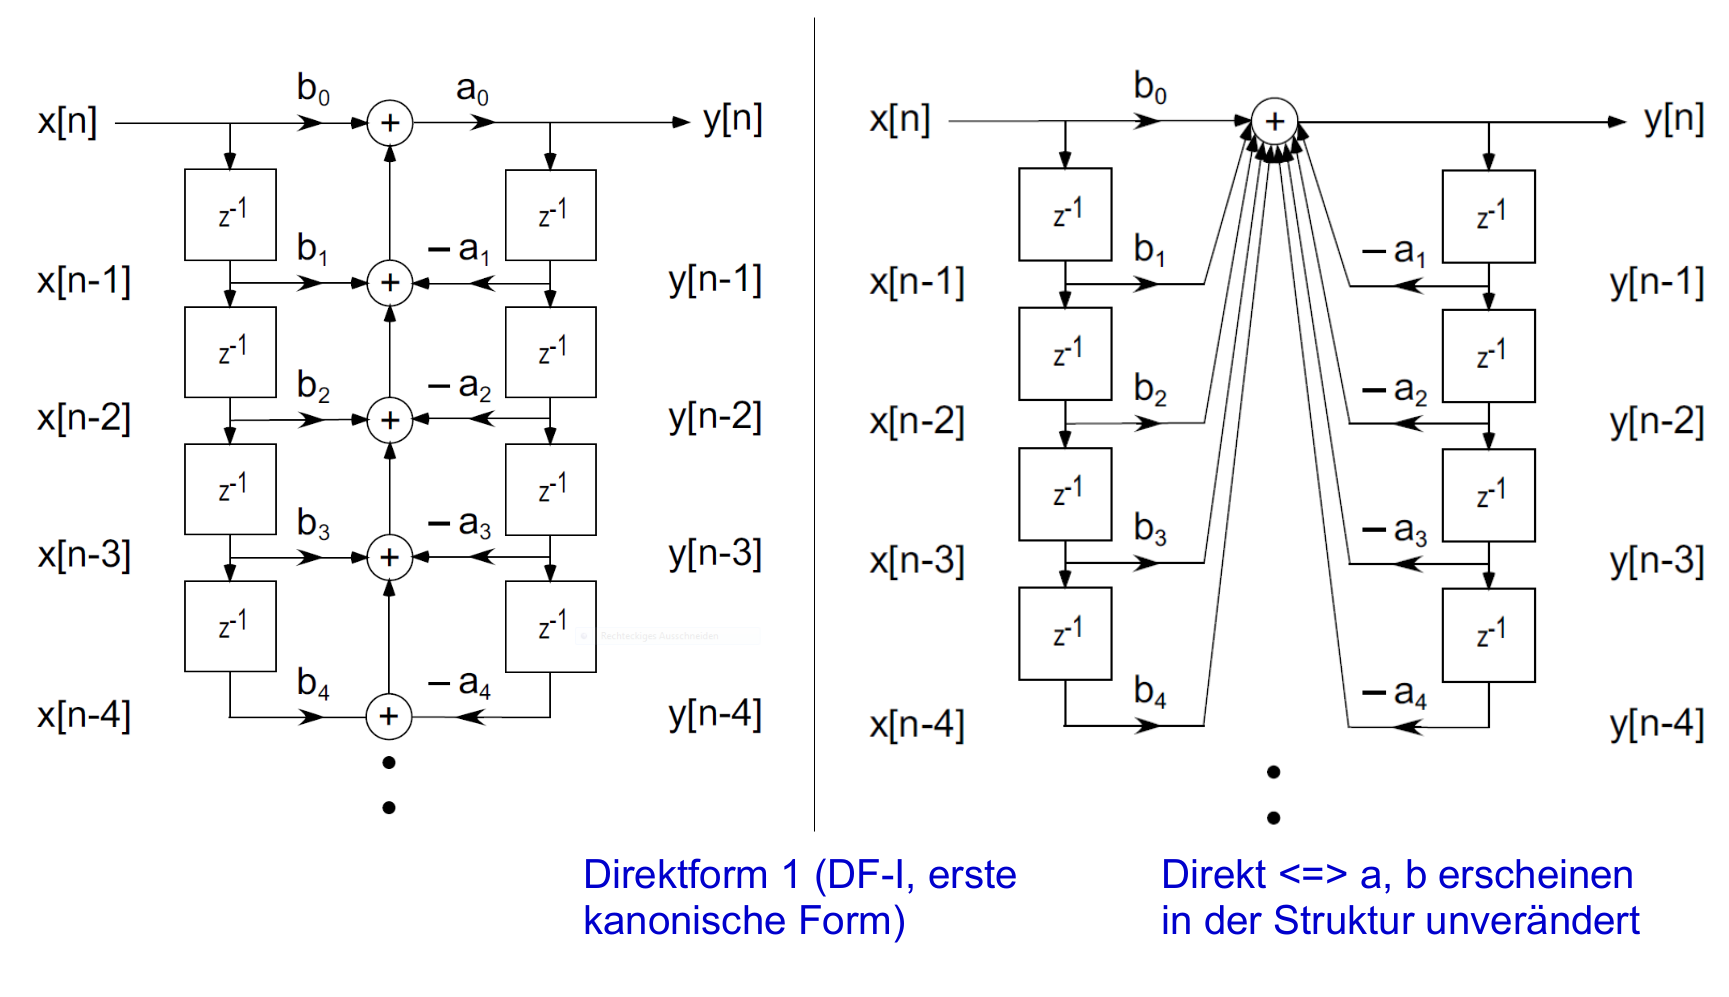
\includegraphics[width=.5\textwidth]{./img/Direktform_1_IIR.png}  
\end{center}  

\textbf{Direktform II:}
\begin{center}
  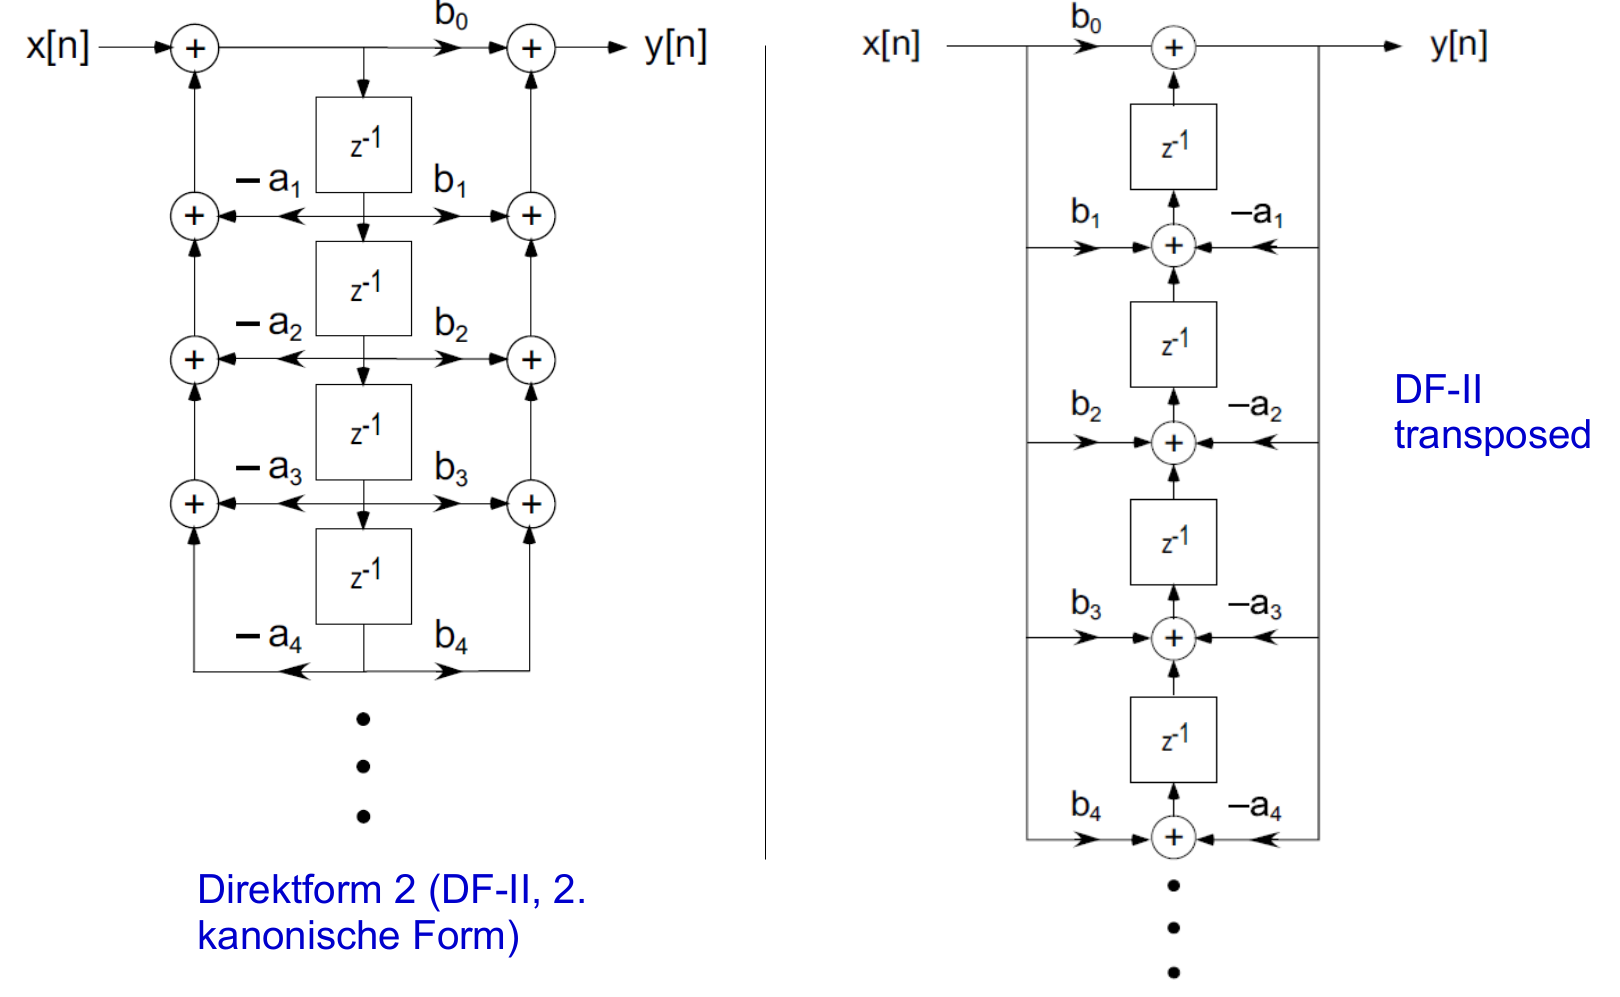
\includegraphics[width=.5\textwidth]{./img/Direktform_2_IIR.png}
\end{center}

\textbf{3. Kanonische Form:}
\begin{center}
  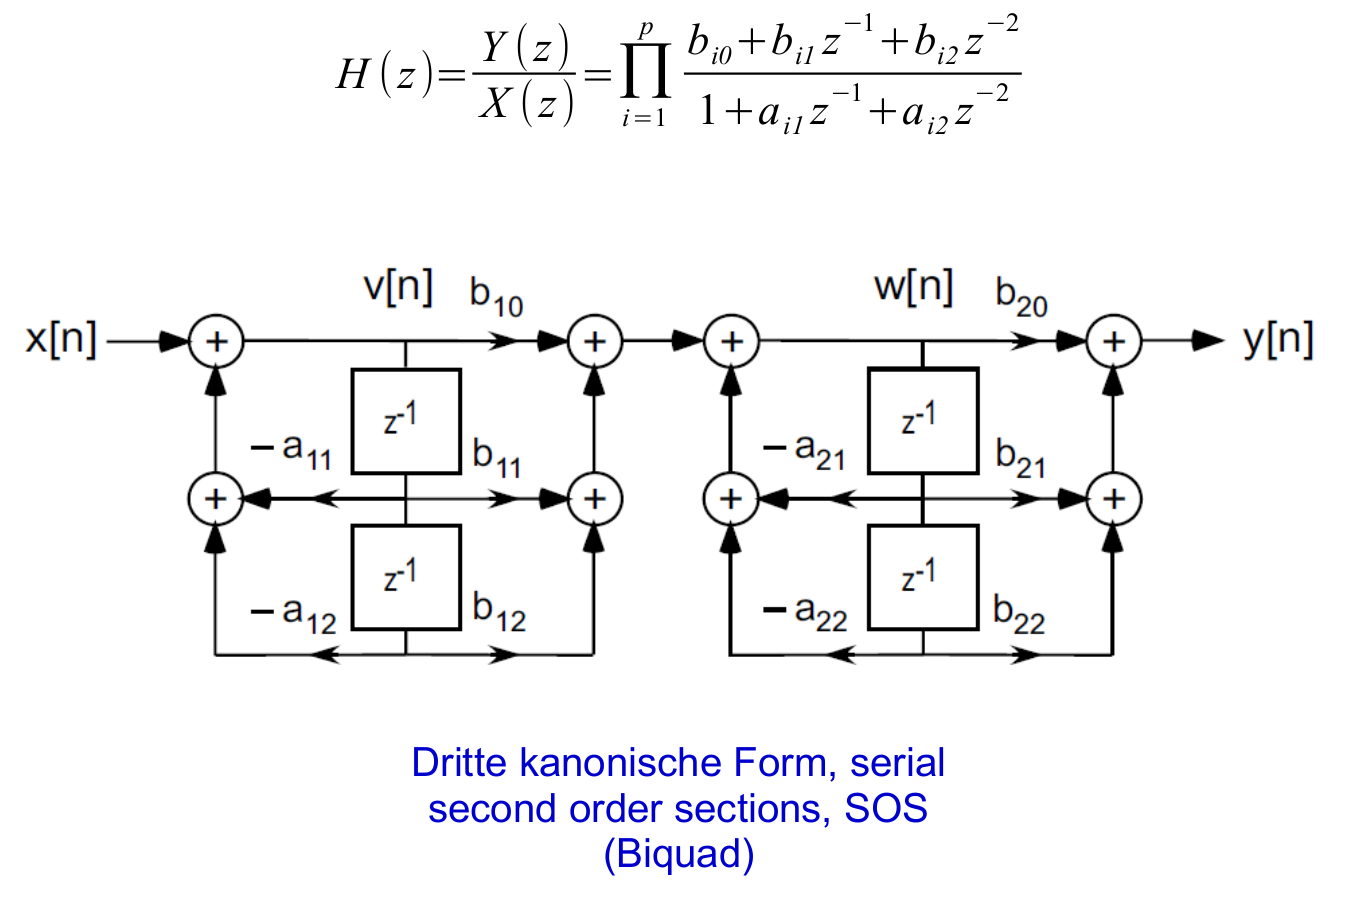
\includegraphics[width=.5\textwidth]{./img/Kanonische_Form_3_IIR.png}
\end{center}

\textbf{4. Kanonische Form:}
\begin{center}
  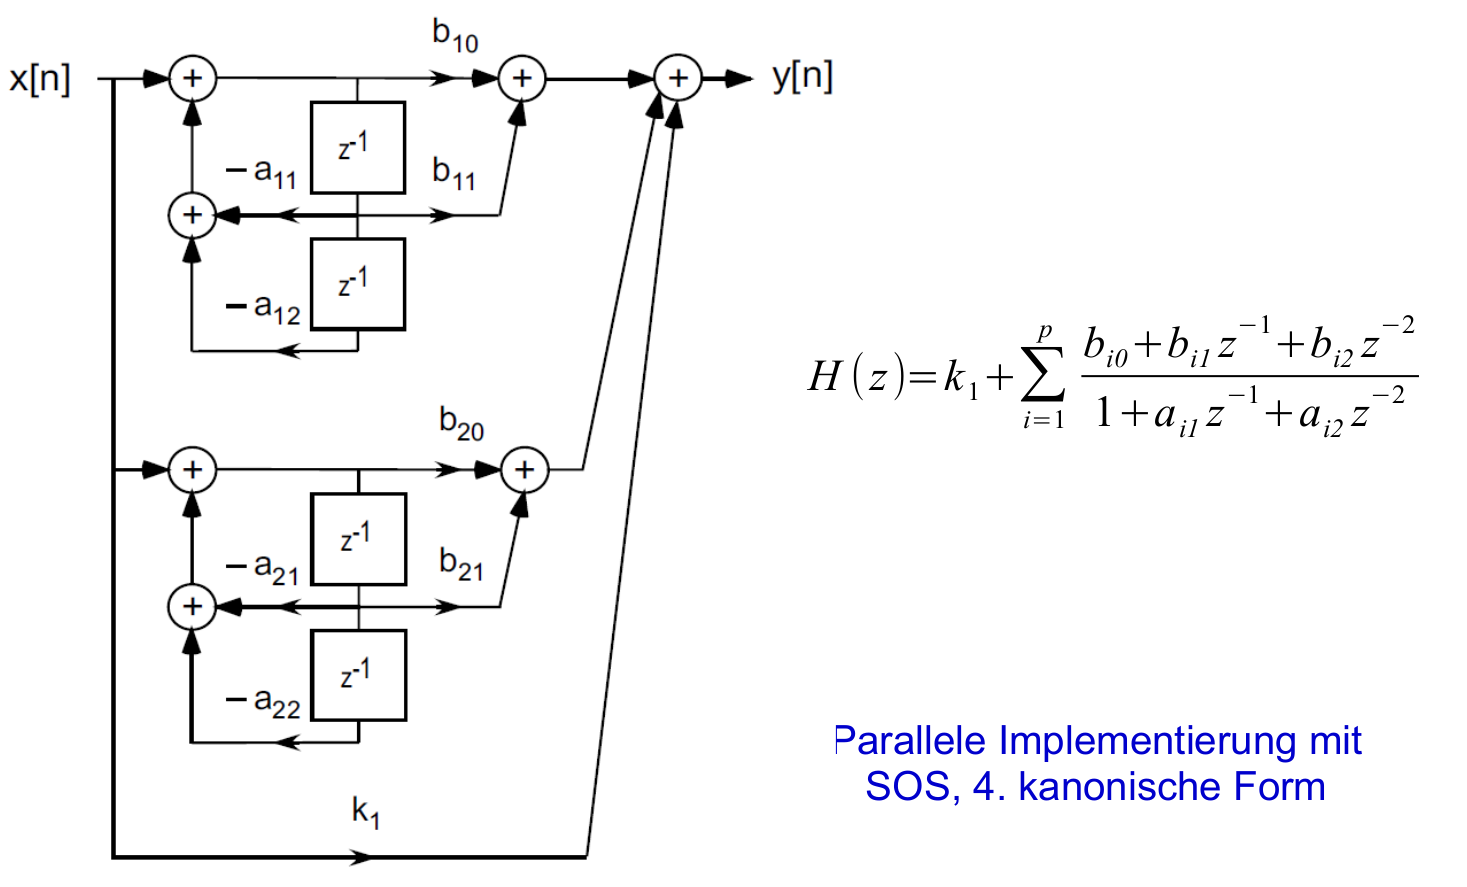
\includegraphics[width=.5\textwidth]{./img/Kanonische_Form_4_IIR.png}
\end{center}

  \begin{mdframed}[style=exercise]
    \begin{align}
        A(0)y(k)=\sum_{i=0}^{N} B(i) x(k-i) - \sum_{i=0}^{N} A(i) y(k-i)
    \end{align}
  \end{mdframed}

\subsubsection{Realisierung des IIR in C:}

\begin{minted}[fontsize=\scriptsize]{c}
void iir()
{
    xLeft[0]  = CodecDataIn.Channel[LEFT] + CodecDataIn.Channel[RIGHT];
    yLeft[0] = 0;                           // initialize the output value

    for (i = 0; i <= N; i++){
        yLeft[0] += B[i] * xLeft[i];
    }
    for (i = 1; i <= N; i++){
        yLeft[0] -=  A[i] * yLeft[i];
    }
    for (i = N; i > 0; i--)
    {
        xLeft[i] = xLeft[i-1];
        yLeft[i] = yLeft[i-1];
    }
    CodecDataOut.Channel[LEFT]  = yLeft[0]; // output the filtered value
}
\end{minted}
% \scalebox{0.85}{
%     \begin{center}
%     \begin{tabular}{ | c | c | c | }
% \cline{1-3}
%         & Zeitbereich & Spektralbereich \\
% \cline{1-3}
%         Linearität & $a\cdot x_1(k) b\cdot x_2(k)$ & $a\cdot X_1(n) +b\cdot X_2(n)$ \\
%     \end{tabular}
%     \end{center}

%%%%%%%%%%%%%%%%%%%%%%%%%%%%%%%%%%%%%%%%%%%%%  Notch %%%%%%%%%%%%%%%%%%%%%%%%%%%%%%%%%%%%%%%%%%%%%%%%%%%%%
\subsection{Notch-IIR-Filter}
\subsubsection{Allgemeines:}
\textbf{SOS-IIR-Notch-Filter (Beispiel):}
\begin{center}
  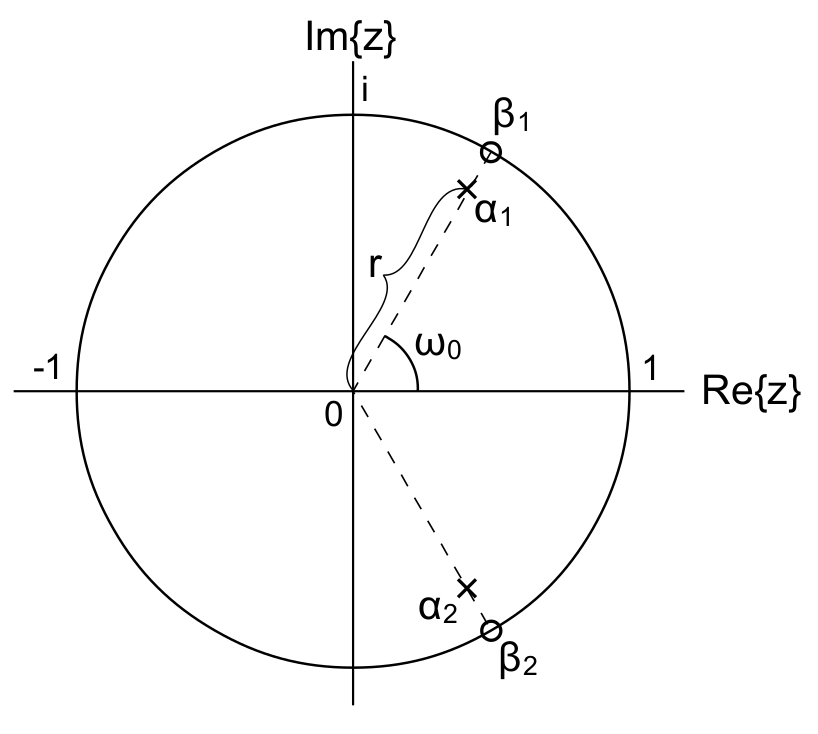
\includegraphics[width=.5\textwidth]{./img/Notch_Filter_SOS.png}
\end{center}

  \begin{mdframed}[style=exercise]
    \begin{align}
  H(z) = k \frac{(z-\beta_1)(z-\beta_2)}{(z-\alpha_1)(z-\alpha_2)} 
       = k \frac{1-2\cos(\omega_0)z^{-1}+z^{-2}}{1-2r\cos(\omega_0)z^{-1}+r^2 z^{-2}}
    \end{align}
  \end{mdframed}
$f_0$ = Kerbfrequenz, $f_s$ = Abtastfrequenz $B_{3dB}$ = Kerbbreite 
  \begin{mdframed}[style=exercise]
    \begin{align}
      k = \frac{1-2r\cos(\omega_0)+r^2}{1-2\cos(\omega_0)+1}\\
      \omega_0 = 2\pi \frac{f_0}{f_s}\\
      r=1-(\frac{B_{3dB}}{f_s})\pi
    \end{align}
  \end{mdframed}

\subsubsection{Anwendungsbeispiel:}
\begin{enumerate}
  \item Ermitteln des spektralen Maximum in durch die FFT generierten Daten
  \item Ermitteln der entsprechenden Störfrequenzen
  \item Errechnen der Koeffizienten des Notch-Filters mit der Störfrequenz als Kerb-Frequenz
  \item Filtern des diskretisierten Signales mit errechnetem Filter
  \item Ausgabe der bearbeiteten Audio-Sequenz
\end{enumerate}

\section{Oszillatoren / Signalgeneratoren}
%%%%%%%%%%%%%%%%%%%%%%%%%%%%%%%%%%%%%%%%%%%%%  IIR-Oszillator %%%%%%%%%%%%%%%%%%%%%%%%%%%%%%%%%%%%%%%%%%%%%%%%%%%%%
\subsection{IIR-Oszillator (Digital Resonator)}
\subsubsection{Allgemeines:}
\begin{itemize}
  \item Oszillator auf Basis einer z-Transformation
  \item Anregung des Systems mit Impuls bei $k=0$
  \item System mit Polen auf Einheitskreis\\
  $\rightarrow$ Grenzstabiles System\\
  $\rightarrow$ System schwingt mit konst. Frequenz
\end{itemize}

\textbf{Vorgehen:}
\begin{enumerate}
  \item z-Transformation des kontinuierlichen Systems
  \item Ausmultiplizieren von $H(z)$ mit $Y(z)$ bzw. $X(z)$
  \item Anwenden von \\
  $Y(z)\cdot z^{-1}=y[n-1]$ bzw. $x(z)\cdot z^{-1}=x[k-1]$
  \item Auflösen nach y(k)
  \item Impuls als Eingangssignal $x[k] = [1, 0, 0, ...]$
\end{enumerate}

\textbf{Vorteil:}
\begin{itemize}
  \item Minimaler Verbrauch von Speicher und Rechenleistung
  \item Anpassbarkeit an beliebige Funktionen
  \item Hohe Auflösung und Flexibilität
\end{itemize}  

\textbf{Nachteil:}
\begin{itemize}
  \item Frequenz muss vor Start festgelegt werden
  \item durch Quantisierung kann Pol aus dem Einheitskreis rutschen und instabil werden
  \item Oszillator muss einschwingen
\end{itemize}  

  \begin{mdframed}[style=exercise]
    \begin{align}
    sin(\omega_0 k) \leftrightarrow \frac{sin(\omega_0)z^{-1}}{1-2\cos(\omega_0)z^{-1}+z^{-2}}\\
    y(n) = sin(\omega_0)x(n-1)+2cos(\omega_0)y(n-1)-y(n-2)
    \end{align}
  \end{mdframed}

\subsubsection{Realisierung des IIR-Oszillators in C:}
  \begin{minted}[fontsize=\scriptsize]{c}
    enum lrtype {LEFT, RIGHT};
    volatile union {unsigned UINT; short Channel[2];}
    CodecDataIn, CodecDataOut;
    float fDesired = 1000; // your desired signal frequency
    float A = 32000; // your desired signal amplitude
    float pi = 3.1415927; // value of pi
    float theta;// digital frequency (omega0 in textbook)
    float y[3] = {0, 1, 0}; // the last 3 output values.
    unsigned fs = 48000; // sample frequency

    void isr_resonator(){
      CodecDataIn.UINT = ReadCodecData(); // get input data samples
      theta = 2 * pi * fDesired / fs; // calc. the digital frequency
      y[0] = 2 * cosf(theta) * y[1] - y[2]; // calculate the output
      y[2] = y[1]; // prepare for the next ISR
      y[1] = y[0]; // prepare for the next ISR
      CodecDataOut.Channel[ LEFT] = A * sinf(theta) * y[0]; // just scale
      CodecDataOut.Channel[RIGHT] = CodecDataOut.Channel[LEFT];
    }

    WriteCodecData(CodecDataOut.UINT);  
  \end{minted}

\subsection{DDS-Oszillator}
\subsubsection{Allgemeines:}
\begin{itemize}
  \item Direct Digital Synthesizer
  \item Errechnen des Funktionsverlaufs
  \item Verwendung von Accumulator und Modulo-Operator
  \item sin() kann berechnet oder mittels Lookup-Table realisiert werden
\end{itemize}

\textbf{Vorteil:}
\begin{itemize}
  \item Kann einfach bei FPGA verwendet werden
  \item Robuster Phasen- oder Frequenzwechsel mit sofortiger Wirkung
  \item kontinuierliche Signalform
  \item keine Einschwingzeit
\end{itemize}  

\textbf{Nachteil:}
\begin{itemize}
  \item Höherer Speicher- und Rechenleistungs-Bedarf
  \item Frequenzauflösung abhängig im Wesentlichen von Auflösung der Lookup ab
\end{itemize}  

\begin{center}
  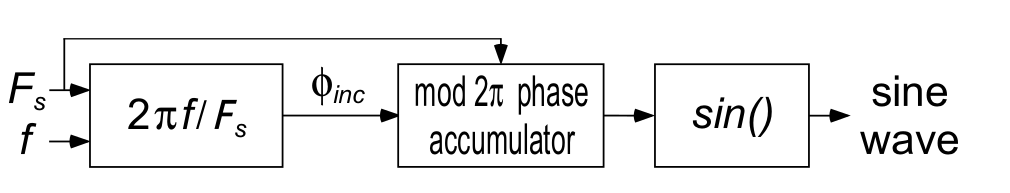
\includegraphics[width=.5\textwidth]{./img/DDS_sin().png}
\end{center} 

\begin{center}
  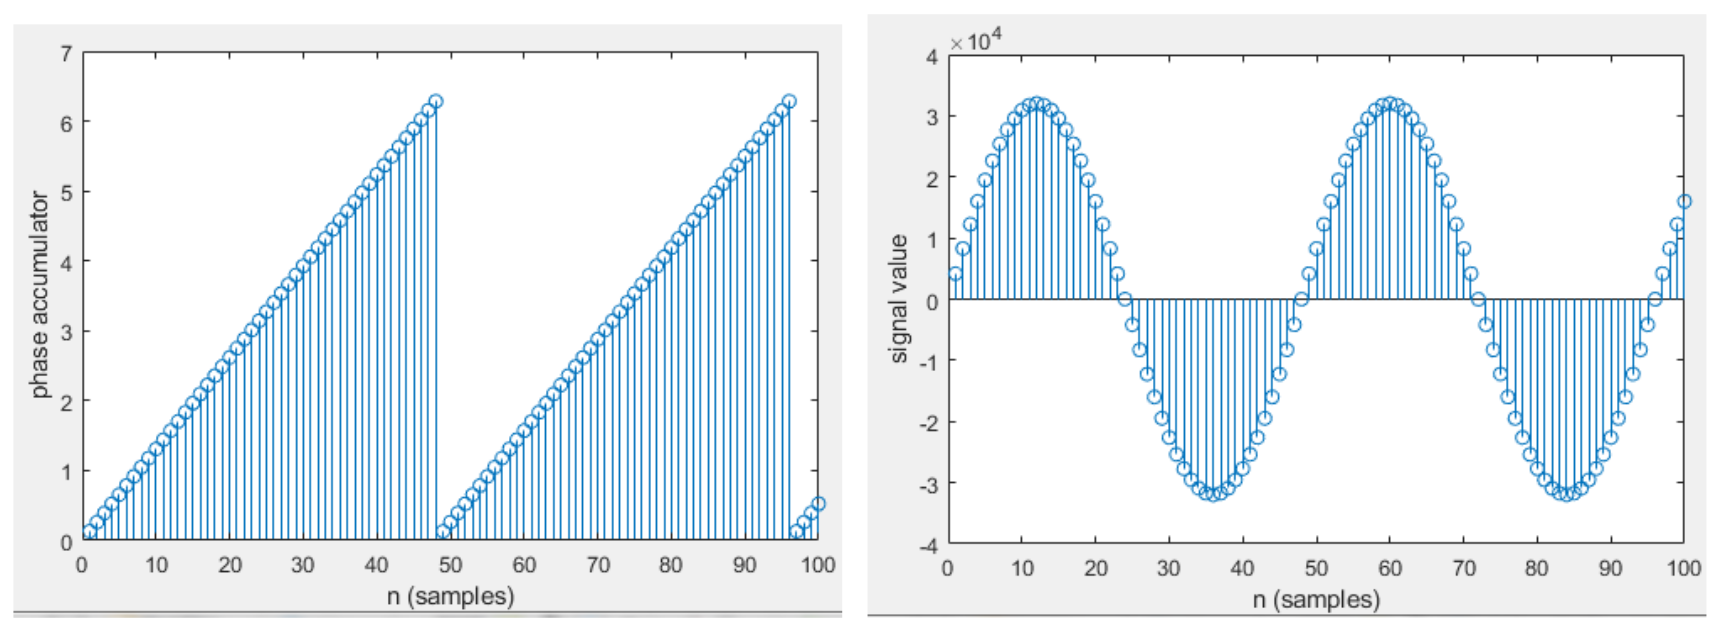
\includegraphics[width=.5\textwidth]{./img/sin_phaseincrement.png}
\end{center} 

  \begin{mdframed}[style=exercise]
    \begin{align}
        \varphi_{inc} = 2\pi\frac{f_0}{f_s}\\
        \varphi = \varphi + \varphi_{inc}\\
        \varphi_{inc} < \pi (sonst Aliasing)\\
        x(n)= Asin(n\varphi)
    \end{align}
  \end{mdframed}

\subsubsection{Realisierung des DDR-Oszillators in C:}
\begin{minted}[fontsize=\scriptsize]{c}
float A = 32000; //signal's amplitude 
float fDesired = 1000; // signal's frequency 
float phase = 0; // signal's initial phase 
float pi = 3.1415927; // value of pi 
float phaseIncrement; // incremental phase 
int fs = 48000; // sample frequency 

void sineGen_ISR(){
CodecDataIn.UINT = ReadCodecData();
// algorithm begins here 
phaseIncrement = 2*pi*fDesired/fs;
phase += phaseIncrement;
if (phase >= 2*pi) phase -= 2*pi;
// get input data samples
// calculate the phase increment 
// calculate the next phase 
// modulus 2*pi operation 
CodecDataOut.Channel[ LEFT] = A*sinf(phase); // scaled L output 
CodecDataOut.Channel[RIGHT] = A*cosf(phase); // scaled R output 
// algorithm ends here 
}

WriteCodecData(CodecDataOut.UINT);
\end{minted}


\subsubsection{Spezialfälle:}
\begin{enumerate}
  \item \textbf{Niquist-Frequenz: }$f=\frac{f_s}{2} \rightarrow \varphi_{inc} = \pi$\\
  $\rightarrow sin(n\cdot\pi) = 0$ bzw. $cos(n\cdot\pi) = [1, -1, 1, -1, ...]$
  \item $f=\frac{f_s}{4} \rightarrow \varphi_{inc} = \frac{\pi}{2}$\\
  $\rightarrow sin(n\cdot\pi) = [0, -1, 0, -1, ...]$\\ 
  $\rightarrow cos(n\cdot\pi) = [1, 0, -1, 0, ...]$
  \item \textbf{$f_s= N \cdot f$ (Ganzzahliges Vielfaches):} \\
  $\rightarrow$ nur N Werte müssen berechnet werden\\
  $\rightarrow$ $cos(\varphi_{inc}\cdot n)$ für n = 0, 1, ..., N
 
\end{enumerate}

%%%%%%%%%%%%%%%%%%%%%%%%%%%%%%%%%%%%%%%%%%%%%  Blocksignalverarbeitung %%%%%%%%%%%%%%%%%%%%%%%%%%%%%%%%%%%%%%%%%%%%%%%%%%%%%
\section{Blocksignalverarbeitung:}
\subsection{Dreifach-Puffer:}
\textbf{Allgemein:}
\begin{itemize}
  \item Kein Kopieren notwendig
  \item 3 unabhängige Buffer nötig
  \item 3 Pointer zeigen welcher Buffer befüllt, verarbeit bzw. entleert wird  
\end{itemize}

  \begin{center}
      \includegraphics[width=.5\textwidth]{./img/frame.png}
  \end{center}
ISR schreibt N samples nach buffer[fill\_index] und setzt ready\_index = fill\_index.\\ 
buffer[fill\_index] ist jetzt dran mit ProcessBuffer.
Jeder Frame generiert einen Interrupt.
  \begin{center}
      \includegraphics[width=.5\textwidth]{./img/buffers.png}
  \end{center}
  Block
\begin{itemize}
    \item fill\_index wird von ADC gefüllt
    \item dump\_index wird an DAC geschrieben
    \item ready\_index Buffer für Blocksignalverarbeitung
\end{itemize}

\subsubsection{Realisierung eines Dreifach-Puffers in C:}
\begin{minted}[fontsize=\scriptsize]{c}
#define BUFFER_LENGTH   	1024	// buffer length in samples 
#define NUM_BUFFERS         3
volatile float buffer[NUM_BUFFERS][2][BUFFER_LENGTH];

void ProcessBuffer()
// Processes the data in buffer[ready_index]
{
    volatile float *pL = buffer[ready_index][LEFT];
    volatile float *pR = buffer[ready_index][RIGHT];
    // Do the Process
    // ...
    buffer_ready = 0;   // means were done here
}

interrupt void Codec_ISR()
{                    
    static Uint8 fill_index = INITIAL_FILL_INDEX; // index of buffer to fill
    static Uint8 dump_index = INITIAL_DUMP_INDEX; // index of buffer to dump
    static Uint32 sample_count = 0; // current sample count in buffer

    // get input data samples
  	CodecDataIn.UINT = ReadCodecData();		
  	// IN
    buffer[fill_index][ LEFT][sample_count] = LEFT + RIGHT; // cropped
    buffer[fill_index][RIGHT][sample_count] = RIGHT + LEFT; // cropped
    // OUT
    CodecDataOut.channel[ LEFT] = buffer[dump_index][LEFT][sample_count];
    CodecDataOut.channel[RIGHT] = buffer[dump_index][RIGHT][sample_count];

    // update sample count and swap buffers when filled 
    if(++sample_count >= BUFFER_LENGTH) {
        sample_count = 0;
        ready_index = fill_index;
        if(++fill_index >= NUM_BUFFERS)
            fill_index = 0;
        if(++dump_index >= NUM_BUFFERS)
            dump_index = 0;
        if(buffer_ready == 1) // set a flag if buffer isn't processed in time 
            over_run = 1;
        buffer_ready = 1;
    }
	WriteCodecData(CodecDataOut.UINT);// send output data to  port
}
\end{minted}

\subsubsection{Blocksignalverarbeitung mit DMA}
\textbf{Vorteil: } Prozessor muss sich nicht mit Befüllen beschäftigen sondern kann verarbeiten\\
$\rightarrow$ Geschwindigkeitsvorteil

\begin{itemize}
    \item DMA kopiert Sample von ADC nach Eingangsbuffer
    \item DMA kopiert Processed von Ausgangsbuffer nach DAC
    \item DMA generiert Interrupt, wenn N Samples transfert wurden $\rightarrow$ Buffer-Swap
\end{itemize}

\begin{minted}[fontsize=\scriptsize]{c}
interrupt void EDMA_ISR()
{
    if(++ready_index >= NUM_BUFFERS)
        ready_index = 0;
    if(buffer_ready ==1) //buffer isnt processed in time
        over_run = 1;
    buffer_ready = 1; //buffer is now ready for processing
}
\end{minted}

\subsection{FIR mit Blocksignalverarbeitung}
\subsubsection{Allgemeines:}
Bsp. Ordnung Filter N = 4, Framesize = 8\\
  \begin{center}
      \includegraphics[width=.25\textwidth]{./img/firframe1.png}
      \includegraphics[width=.25\textwidth]{./img/firframe2.png}
  \end{center}
\textbf{Problem:} Die Start und Endzustände müssen jeweils berücksichtigt werden, um den FIR korrekt zu implementieren.\\ 
$\rightarrow$ Bei Frame-Übergängen müssen die N-1 letzten Werte des letzten Frames berücksichtigt werden.\\
$\rightarrow$ Audiotechnisch würde dies ein \grqq{}Knacken-\grqq{} und \grqq{}Klicken\grqq{} hervorrufen
\textbf{Lösung:} Der Puffer muss groß genug sein, um sowohl die Frame-Werte als auch die nötigen Randwerte speichern zu können (Framesize += N).


\begin{itemize}
    \item Left[N|FRAMESIZE], buffer[FRAMESIZE]
    \item Left[N:FRAMESIZE+N] = buffer[0:FRAMESIZE]
    \item buffer[0:FRAMESIZE] = Left * B (B wird \\drüber FRAMESIZE-mal drüber geschoben s.o)
    \item Left[0:N] = Left[FRAMESIZE:FRAMESIZE+N]
\end{itemize}

\subsubsection{Realisierung eines FIR mit Blocksignalverar. in C:}
\begin{minted}[fontsize=\scriptsize]{c}
void ProcessBuffer()
{
    short *pBuf = buffer[ready_index];
    // extra buffer room for convolution "edge effects"
    // N is filter order from coeff.h
    static float Left[BUFFER_COUNT+N]={0}, Right[BUFFER_COUNT+N]={0};
    float *pL = Left, *pR = Right;
    float yLeft, yRight;
    int i, j, k;
    // offset pointers to start filling after N elements

    pR += N;
    pL += N;

    // extract data to float buffers
    for(i = 0; i < BUFFER_COUNT; i++) 
    { 
        *pR++ = *pBuf++;
        *pL++ = *pBuf++;
    }
    // reinitialize pointer before FOR loop
    pBuf = buffer[ready_index];

    // Implement FIR filter
    for(i=0; i < BUFFER_COUNT; i++) 
    {
        yLeft = 0; // initialize the LEFT output value
        yRight = 0; // initialize the RIGHT output value

        for(j=0,k=i+N; j <= N; j++,k--) 
        {
            yLeft += Left[k] * B[j]; // perform the LEFT dot-product
            yRight += Right[k] * B[j]; // perform the RIGHT dot-product
        }
        // pack into buffer after bounding (must be right then left)
        *pBuf++ = _spint(yRight * 65536) >> 16;
        *pBuf++ = _spint(yLeft * 65536) >> 16;
    }

    // save end values at end of buffer array for next pass
    // by placing at beginning of buffer array
    for(i=BUFFER_COUNT,j=0; i < BUFFER_COUNT+N; i++,j++) 
    {
        Left[j] = Left[i];
        Right[j] = Right[i];
    }
    buffer_ready = 0; // signal we are done
}
\end{minted}

%%%%%%%%%%%%%%%%%%%%%%%%%%%%%%%%%%%%%%%%%%%%%  Ping-Pong %%%%%%%%%%%%%%%%%%%%%%%%%%%%%%%%%%%%%%%%%%%%%%%%%%%%%
\subsubsection{Allgemein:}
\textbf{Vorteile:}
\begin{itemize}
  \item Kein Kopieren zu Float-Arrays
  \item Robuste Buffer-Identifizierung, die Breakpoints unterstützt
\end{itemize}

\textbf{Nachteile:} Aufwendiges Schieben in dem Filterspeicher

  \begin{center}
      \includegraphics[width=.35\textwidth]{./img/pingpong.png}
  \end{center}
  \begin{itemize}
    \item gleiche Latenz (=Durchlaufzeit 2 Buffer)
    \item Ping-Pong einfacher zu verwalten mit DMA
  \end{itemize}

%%%%%%%%%%%%%%%%%%%%%%%%%%%%%%%%%%%%%%%%%%%%%  FFT %%%%%%%%%%%%%%%%%%%%%%%%%%%%%%%%%%%%%%%%%%%%%%%%%%%%%
\section{FFT}
Die FFT basiert auf dem \textbf{Devide-and-Conquer} Prinzip,
sodass schon berechnete Zwischenergebnisse wiederverwendet werden.
Mögliche Realisierungsformen:
\begin{itemize}
    \item Decimation in Frequency
    \item Decimation in Time 
\end{itemize}
  \begin{mdframed}[style=exercise]
    \begin{align}
        w_N^{nk}&=e^{-j\frac{2\pi nk}{N}}\\
        w_N^{2nk}&=e^{-j\frac{4\pi nk}{N}}=w_{\frac{N}{2}}^{nk}
    \end{align}
  \end{mdframed}
\subsection{Decimation in Time (DIT)}
1. Aufteilung in $Y(n) = Y_{even}(n)+Y_{odd}(n)$
  \begin{mdframed}[style=exercise,font=\scriptsize]
    \begin{align}
        Y(n)&=\sum_{k=0}^{N/2-1} y(2k)w_N^{2nk}+\sum_{k=0}^{N/2-1} y(2k+1)w_N^{(2k+1)n}\\
        Y(n)&=\sum_{k=0}^{N/2-1} y(2k)w_N^{2nk}+w_N^{n}\sum_{k=0}^{N/2-1} y(2k+1)w_N^{2kn}\\
        Y(n)&=\sum_{k=0}^{N/2-1} y(2k)w_{\frac{N}{2}}^{nk}+w_N^{n}\sum_{k=0}^{N/2-1} y(2k+1)w_{\frac{N}{2}}^{nk}\\
    \end{align}
  \end{mdframed}
2. Aufteilung in $Y(n) = Y_{left}(n)+Y_{right}(n)$
  \begin{mdframed}[style=exercise,font=\scriptsize]
    \begin{align}
        Y(n)&=\sum_{k=0}^{N/2-1} y(2k)w_{\frac{N}{2}}^{nk}+w_N^{n}\sum_{k=0}^{N/2-1} y(2k+1)w_{\frac{N}{2}}^{nk}\\
        Y(n+\frac{N}{2})&=\sum_{k=0}^{N/2-1} y(2k)w_{\frac{N}{2}}^{(n+\frac{N}{2})k}+w_N^{n+\frac{N}{2}}\sum_{k=0}^{N/2-1} y(2k+1)w_{\frac{N}{2}}^{(n+\frac{N}{2})k}
    \end{align}
  \end{mdframed}
mit 
  \begin{mdframed}[style=exercise]
    \begin{align}
        w_{\frac{N}{2}}^{(n+\frac{N}{2})k} &= w_{\frac{N}{2}}^{nk} \cdot \underbrace{w_{\frac{N}{2}}^{k\frac{N}{2}}}_{=1} = w_{\frac{N}{2}}^{nk}\\
        w_N^{n+\frac{N}{2}} &= w_N^n \cdot \underbrace{w^{\frac{N}{2}}_N}_{=-1} = -w_N^n
    \end{align}
  \end{mdframed}
folgt 
  \begin{mdframed}[style=exercise,font=\scriptsize]
    \begin{align}
        Y(n)&=\sum_{k=0}^{N/2-1} y(2k) w_{\frac{N}{2}}^{nk} + w_{\frac{N}{2}}^{n} \sum_{k=0}^{N/2-1} y(2k+1)w_{\frac{N}{2}}^{kn}\\
        Y(n+\frac{N}{2})&=\sum_{k=0}^{N/2-1} y(2k) w_{\frac{N}{2}}^{nk} - w_{\frac{N}{2}}^{n} \sum_{k=0}^{N/2-1} y(2k+1)w_{\frac{N}{2}}^{kn}
    \end{align}
  \end{mdframed}
  \begin{mdframed}[style=exercise]
    \begin{align}
        Y_{left}(n) &= Y_{even}(n) + w_{\frac{N}{2}}^{n} Y_{odd}(n)\\ 
        Y_{right}(n) &= Y_{even}(n) - w_{\frac{N}{2}}^{n} Y_{odd}(n)
    \end{align}
  \end{mdframed}
Die Komplexität ist $O(N\log_2(N))$:\\ 
Es gibt 2 $log_2(N)$ Splitting-Steps mit je $O(n)$

%%%%%%%%%%%%%%%%%%%%%%%%%%%%%%%%%%%%%%%%%%%%%  NCO %%%%%%%%%%%%%%%%%%%%%%%%%%%%%%%%%%%%%%%%%%%%%%%%%%%%%
\section{NCO}
NCO = Counter, der Jeden Takt um ein Phaseninkrement $\mu$ (hier 32) erhöht wird.
Der Ausgang des Counters wird mit LUT in Signalform (sin,cos,sägezahn) umgewandelt. 
Die LUT ist mit $N = 2^n$ 12-bit breiten Werten gefüllt 
  \begin{center}
      \includegraphics[width=.35\textwidth]{./img/nco.png}
  \end{center}
  \begin{mdframed}[style=exercise]
    \begin{align}
        \mu = N \frac{f_d}{f_s}  
    \end{align}
  \end{mdframed}

%%%%%%%%%%%%%%%%%%%%%%%%%%%%%%%%%%%%%%%%%%%%% Nützliche Code-Stückchen %%%%%%%%%%%%%%%%%%%%%%%%%%%%%%%%%%%%%%%%%%%%%%%%%%%%%
\section{Nützliche Code-Ausschitte:}
\textbf{Maximalwert-Ermittlung z.B. für Sepktralauswertung:}
\begin{minted}[fontsize=\scriptsize]{c}
max_value = 0 ; //Startwert des Vergleichs
max_idx = 2 ; //Startindex des Vergleichs
for(int i = 2; i<(N-1); i++){ 
  if( y[i] > max_value){
    max_value = y[i];
    max_idx = i;
  }
}
\end{minted}

\end{document}
